% !TEX root = "/expose_sebastian_keil/expose.tex"

\documentclass[12pt, oneside, paper=A4, DIV=15, ngerman]{scrartcl}
% \usepackage[english]{babel}

%for google fonts
\usepackage{parskip}
\usepackage{fontspec}
\setmainfont{Roboto}[
    Path=./font/Roboto/,
    Extension = .ttf,
    UprightFont=*-Regular,
    BoldFont=*-Bold,
    ItalicFont=*-Italic,
    BoldItalicFont=*-BoldItalic
    ]
\usepackage{float}

% \usepackage{fancyhdr}
% \pagestyle{fancy}
% \fancyhf{} % Clear all header and footer fields
% %\renewcommand{\headrulewidth}{0pt} % No horizontal line in header
% \fancyhead[C]{"Comparative Analysis of the BIWaM and ODOG Models: Identifying structural and behavioural differences and parallels" TBD} % Centered header text
% \newcommand{\helv}{\fontsize{7}{9}\selectfont}


% Setzt die Einrückung auf 2em, du kannst diesen Wert anpassen
\setlength{\parindent}{2em} 

\usepackage[english]{babel}
\usepackage[utf8]{inputenc}

% \usepackage{float} % For multiple figures in one
% \usepackage[caption = false]{subfig}

\usepackage{subcaption} % For multiple figures in one

\usepackage{graphicx} % For including images
\usepackage{caption} % For caption customization
\DeclareCaptionFormat{myformat}{\fontsize{10}{10}\selectfont#1#2#3}
\captionsetup{format=myformat}


% Schriftart
%\usepackage{arev}
%\usepackage[T1]{fontenc}

%Schriftart
%\usepackage{libertine}
%\usepackage{libertinust1math}
%\usepackage[T1]{fontenc}

% Mathe, Symbole, Einheitendarstellung, Chemie
\usepackage{siunitx}  

% Typographie
\usepackage[auto]{microtype}

% Autorenangaben
\usepackage[german]{authblk}
\renewcommand\Authand{, }
\renewcommand\Authands{, }

%Paket zur Erstellung von Gantt-Charts
\usepackage{pgfgantt}

% Darstellung der Literaturangaben
\usepackage[
backend=biber,
style=apa,
sortcites=true,
sorting=nyt,
% citestyle=apa,
% maxbibnames=2,
% firstinits=true
]{biblatex}

\setlength\bibitemsep{2\itemsep}


% Speicherort der Literaturangaben (*.bib Datei)
\bibliography{literatur/refs}

% pdf-Einstellungen
% Angaben ggf. aktualisieren!
\usepackage[
pdftitle={},
pdfsubject={},
pdfauthor={},
pdfkeywords={},  
% Links nicht einrahmen
hidelinks
]{hyperref}


\subject{Bachelor Thesis}
%\title{How the differences between the ODOG and BIWAM models are relating to other findings in vision research?}
\title{Comparison of two multiscale spatial filtering models}
\author[]{Sebastian Keil}
% \author[]{Dr. Joris Vincent}
\affil[]{TU Berlin, Computer Engineering B.Sc.}
\author[]{Supervisor: Dr. Joris Vincent}
\affil[]{TU Berlin, Computational Psychology}
% \affil[2]{TU Berlin, Computational Psychology, Marchstraße 23, 10587 Berlin}
\date{\today}

\begin{document}

\maketitle
\thispagestyle{empty}

%how to quote: ~\parencite{ebel2009}

\renewcommand*\contentsname{Summary}
\tableofcontents

\raggedright
\newpage

\setcounter{page}{1}
\section{Introduction}
\subsection{Light and the Visual System}

In the environment, light is emitted by a source of illumination, such as the sun. Any
surface on which this light falls will reflect a portion of it as \emph{luminance}. This
portion is called the \emph{reflectance} of the surface. The luminance is therefore the
result of \emph{illuminance} and reflectance, as shown in Figure \ref*{fig:figure1} a). A
lightmeter can measure the amount of luminance reflected by a surface, but it cannot tell
what the reflectance of this surface is, because the luminance could be the product of any
combination of illuminance and reflectance.
\begin{equation}
    L = I \cdot R
    \label{eq:lightness_model}
\end{equation} 
The formula \ref*{eq:lightness_model} shows the problem from a mathematical perspective.
\(L\) represents luminance, \(I\) and \(R\) illuminance and reflectance, respectively. It
is simply impossible to solve for \(I\) and \(R\), when only \(L\) is been measured, since
for every \(R\) there is an \(I\) to produce the measured \(L\) \parencite{adelson2000}.
\\ 
However, the human visual system can solve this problem. It is also processing only
luminance, yet it is able to generate the perception of reflectance, which is referred to
as lightness. Figure \ref*{fig:figure1} b) shows an abstraction of this process.

\begin{figure}[H]
\centering
\centering
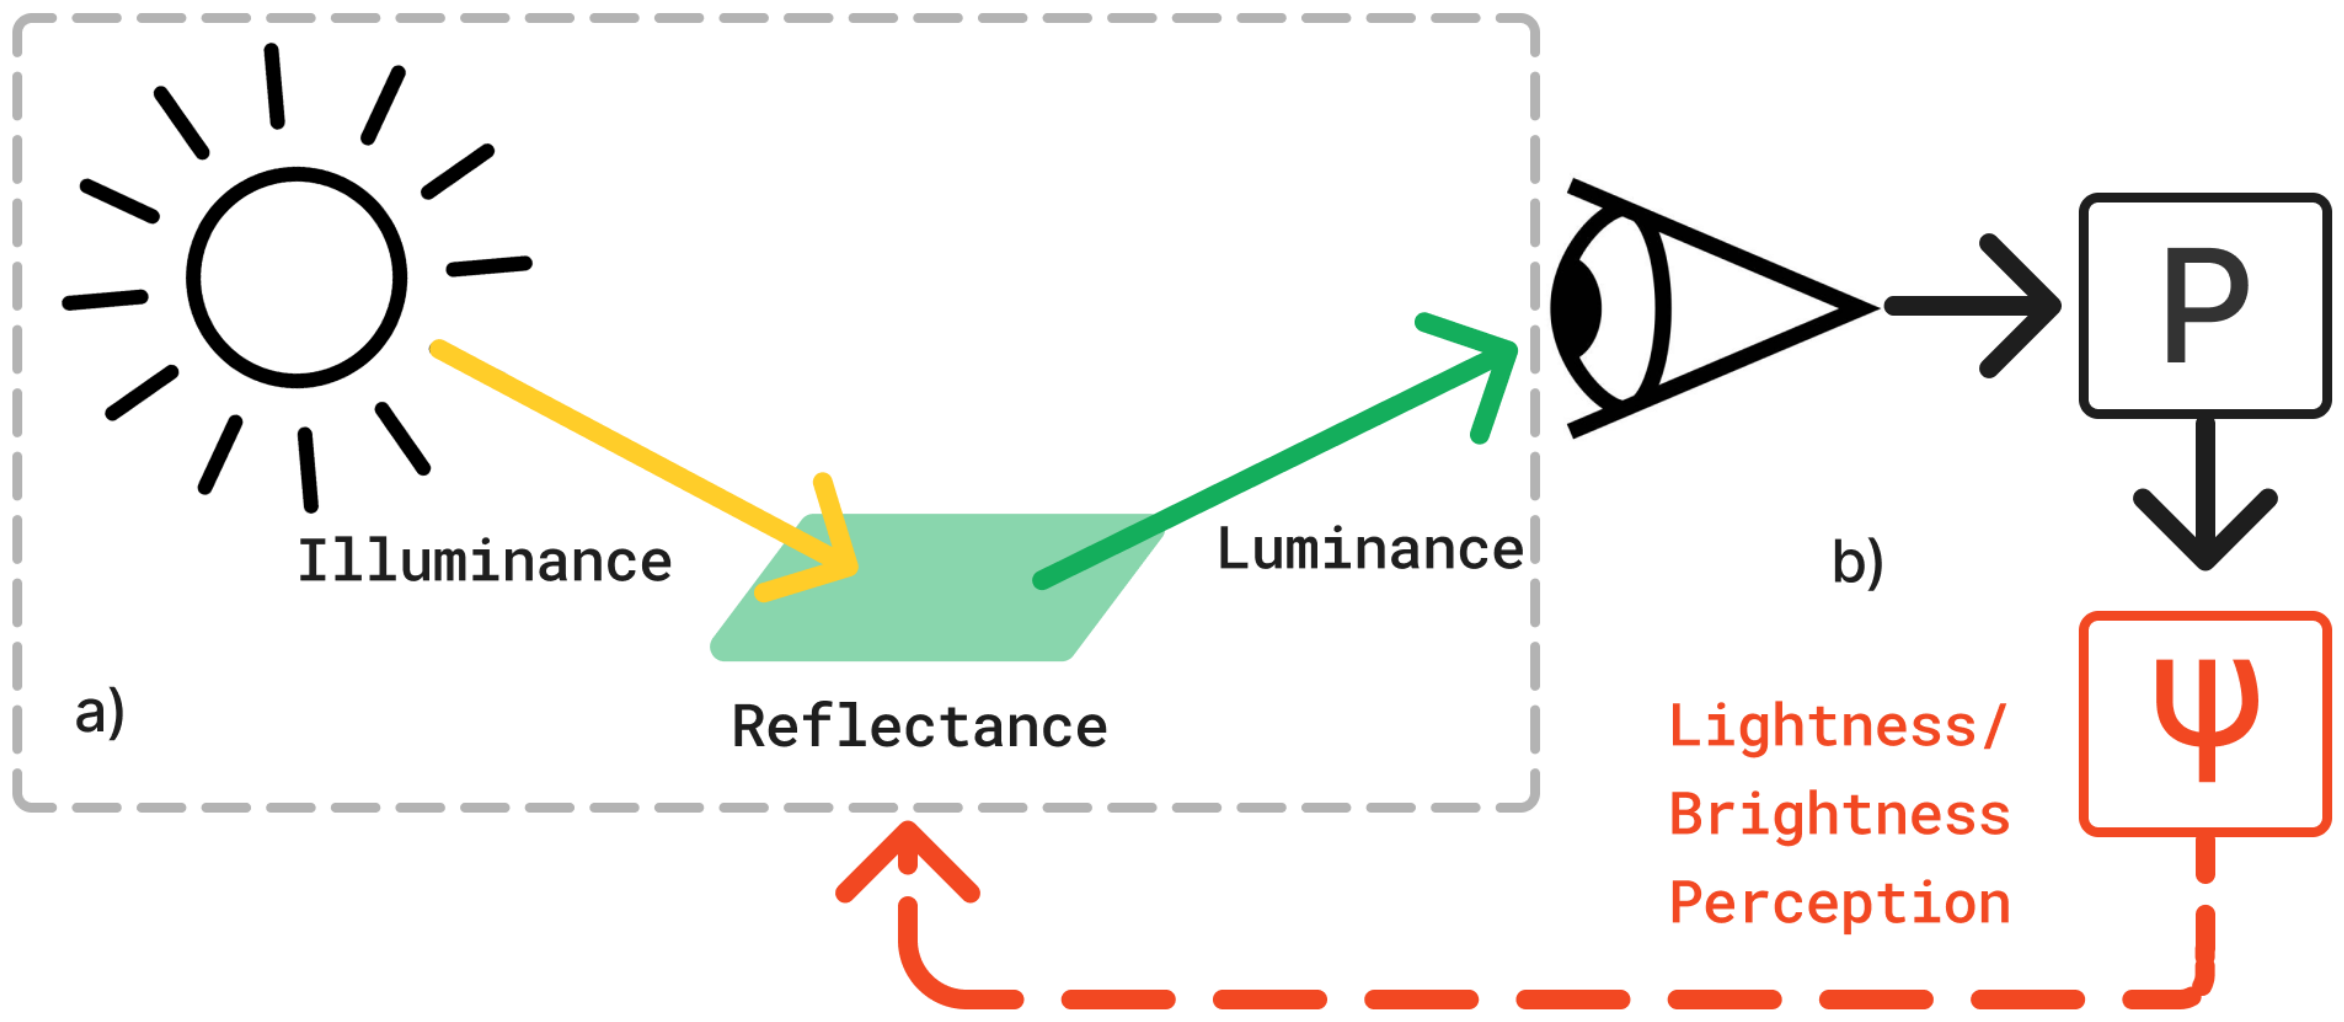
\includegraphics[width=0.9\textwidth]{media/lightness_color.png}
\begin{minipage}{0.8\textwidth}
\caption{a) Relationship between illuminance, reflectance and luminance. Luminance is the
result of illuminance and reflectance. b) The human visual system processes luminance
through an unidentified mechanism, represented by P which is determining lightness and
brightness perception ψ of the surface.}
\label{fig:figure1}
\end{minipage}
\end{figure}

Next to lightness, humans also perceive brightness, which is the perception of luminance,
seen in Figure \ref*{fig:figure1} b). Unlike reflectance, luminance is directly available
at the retinal image and brightness could in principle be derived from the retinal
measurement. However, the visual system does not only consider the corresponding
luminances when evaluating the perceived lightness and brightness of image areas, it also
takes into account the luminances of the surrounding regions \parencite{Kingdom1997}. As a
result the perception can differ from the actual retinal information. The mechanisms
through which the visual system accomplishes these tasks are the subject of current
research and will be discussed further in the following sections.
\newpage

\begin{figure}[H]
    \centering
    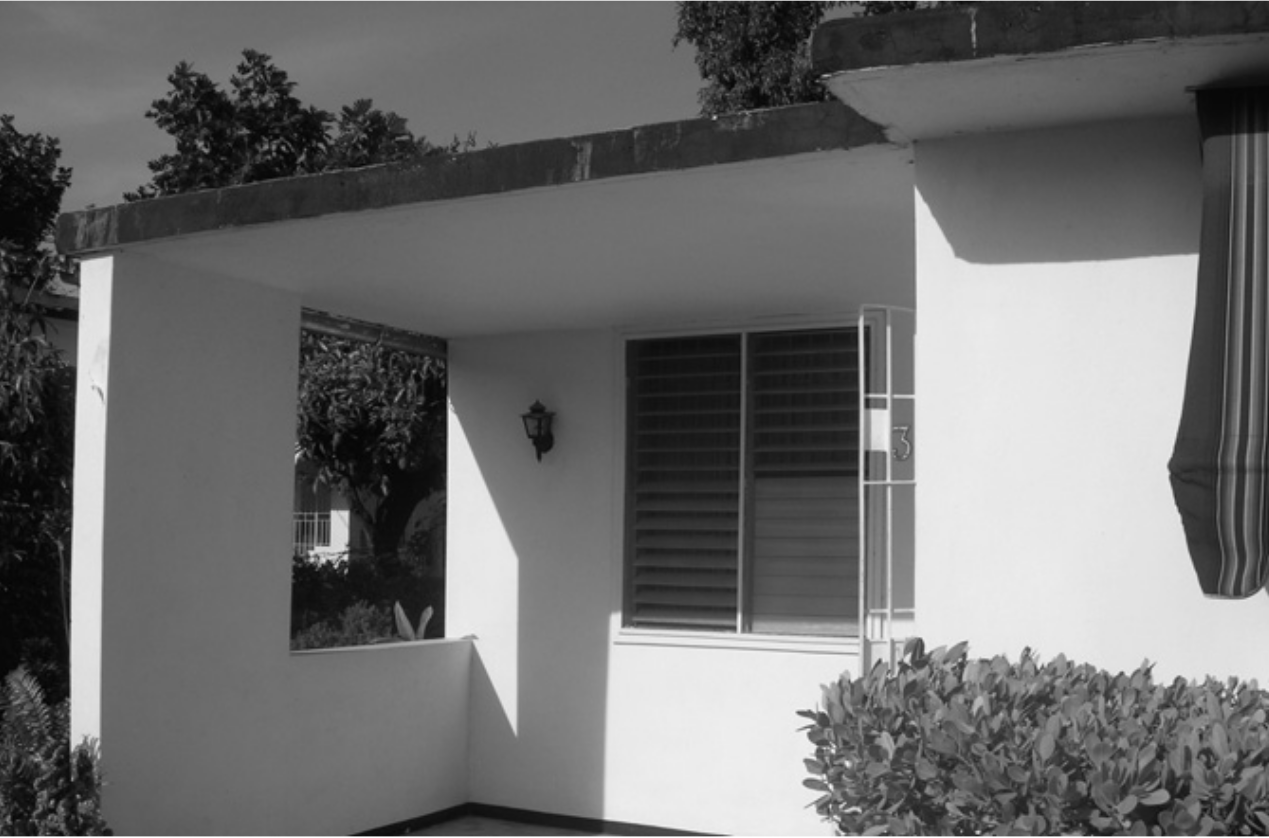
\includegraphics[width=0.7\textwidth]{media/bright_lightness.png}
    \begin{minipage}{0.8\textwidth}
    \caption{Lightness and brightness are distinguishable when illumination is visible.
    \emph{"The walls of the house appear uniformly white — a lightness judgment — yet are
    brighter in some places than others — a brightness judgment"}. Quote and picture from
    Kingdom \parencite*{Kingdom2014}.}
    \label{fig:figure2}
    \end{minipage}
\end{figure}


The distinction between lightness and brightness becomes apparent when information about
illumination is visible, as seen in Figure \ref*{fig:figure2}. \emph{"The walls of the
house appear uniformly white — a lightness judgment — yet are brighter in some places than
others — a brightness judgment"} \parencite{Kingdom2014}. This distinction is important
because brightness is about the relationship between the object and its environment. In
other words, it reveals how the object is exposed to illumination. Lightness, on the other
hand, represents the intrinsic properties of the object, such as color, regardless of the
environment.

Since reflectance is only implicitly perceivable, it can lead to uncertain situations. For
instance, a shadow can dim an area so that a white surface within the shadow reflects the
same amount of light as a black surface in full illumination next to it. Despite this,
human observers can usually distinguish between the white and the black surface
\parencite{arend1993}. 

This phenomenon is illustrated by Edward H. Edelson's \emph{checkerboard shadow illusion},
shown in Figure \ref*{fig:figure3}. The two patches A and B on the checkerboard in Figure
\ref*{fig:figure3}a appear to have different colors, even though they are emitting the
same light, as shown in Figure \ref*{fig:figure3}b.

The cylinder seems to cast a shadow, even though there is no real light source, since the
image is just a two-dimensional representation of the scene. However, the visual system is
designed to process images coming from three-dimensional scenes with illumination and
shadows and so it processes the checkerboard shadow illusion with all the available
information about depth and illumination. To logically follow the processing, one can say,
that patch B reflects the same amount of light as patch A (seen in Figure
\ref*{fig:figure3}b), but is located in the shadow of the cylinder and therefore must have
a higher reflectance. In other words, the visual system needs to react to differences in
illumination and compensate for them in order to estimate the reflectance. This behavior
ensures that the perception of a scene is closely related to the reflectance of its
surfaces and is largely unaffected by the illumination. 

\begin{figure}[H]
    \centering
    \centering
    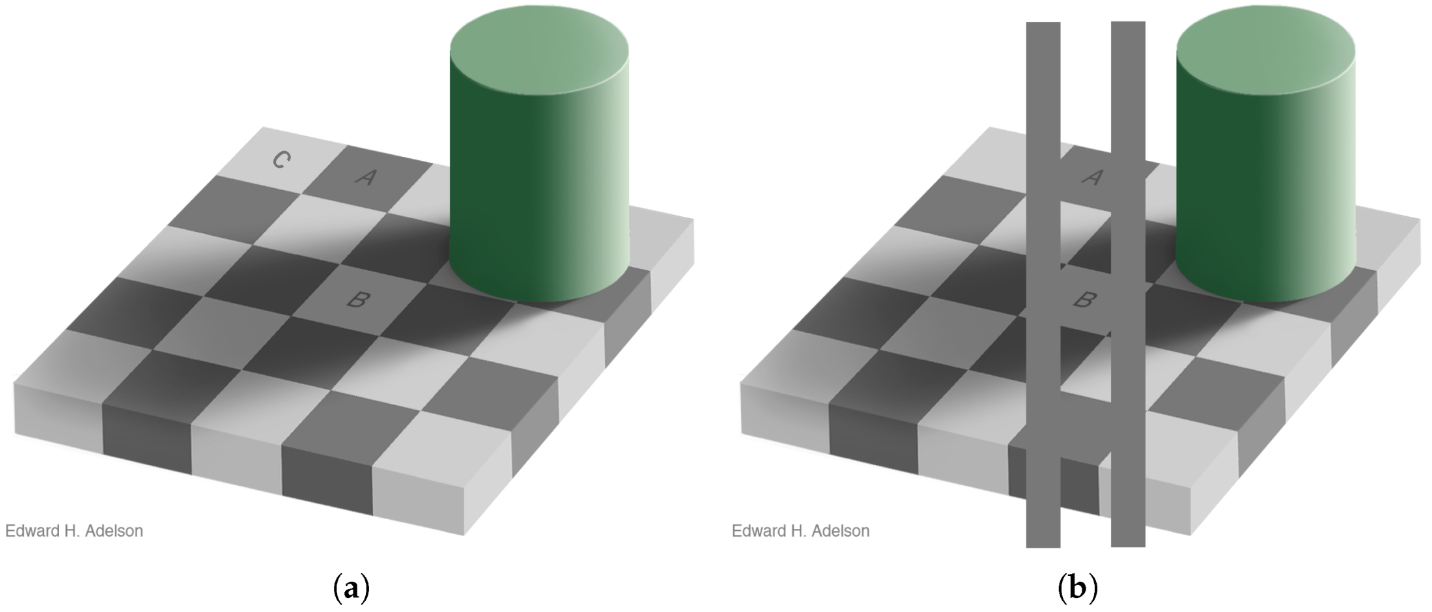
\includegraphics[width=0.85\textwidth]{media/checkershadow_double_full_.png}
    \begin{minipage}{0.8\textwidth}
    \caption{(a) The Checkerboard shadow illusion image; (b) proof image
    \parencite{adelson1995checkershadow}.}
    \label{fig:figure3}
    \end{minipage}
\end{figure}

In everyday life, illusions in brightness and lightness perception are rare, likely due to
the vast amount of information that the visual system can make use of. Shading, shadowing,
and spatial depth can guide the perception of brightness and lightness, like in the
checkerboard shadow illusion. However, there are illusions with less information available
for the visual system, which need a different explanation.

\subsection{Low-Level Vision}

One very simple illusion is the classic \emph{simultaneous contrast illusion}, as seen in
the upper part of Figure \ref{fig:figure4}. Two identical grey squares appear to be
different in brightness, depending on their surroundings. The lack of information about
illumination and spatial depth is crucial in comparison with the checkerboard shadow
illusion. The parts of the visual system, which are processing illumination or spatial
depth, will have no information available in the simultaneous contrast illusion. Here the
idea of detecting illumination and compensating for it will fail, hence a different
explanation is needed.

An explanation for the simultaneous contrast illusion is offered by neural units in the
retina. Hering (1834 —1918) was the first describing their \emph{center surround fields},
which compare luminance areas with their surrounding areas. With that
they could account for the simultaneous contrast illusion. The lower part in Figure
\ref{fig:figure4} illustrates the principle. The blocks under the illusion represent
neurons responding to areas of the illusion image. The surrounding blocks subtract and the
center block adds their responses to the fourth block underneath. When the surrounding
blocks are sensing the darker surrounding of the left patch, their response is small and
so the subtraction is small. As a result the left summing block receives a higher
response, correlating with a human observer experiencing the left patch to be brighter. On
the right patch the surrounding blocks are sensing bright surroundings and so the
subtraction is higher and the summing block receives a lower response, also correlating
with a human observer experiencing the right patch to be darker.


\begin{figure}[H]
    \centering
    \centering
    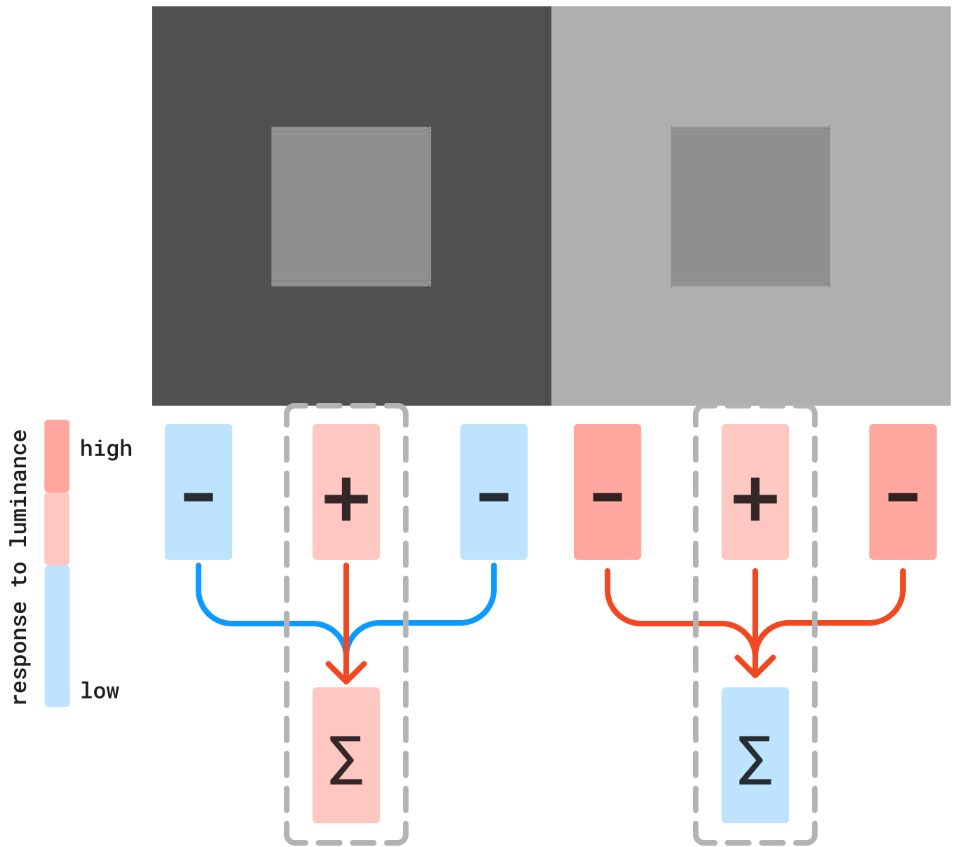
\includegraphics[width=0.75\textwidth]{media/centre_surround.png}
    \begin{minipage}{0.8\textwidth}
    \caption{Above: The simultaneous contrast effect. Two identical grey patches appear to
    be different in brightness, depending on their surrounding. The left patch appears
    brighter than the right patch. \\ Below: The principle of center surround fields. The
    blocks on each side represent neurons, where the surrounding blocks subtract and the
    center block adds their responses to the fourth block underneath. On the left side the
    center response is medium (light red), corresponding to the left patch in the
    illusion, while the surround response is low, corresponding to the surrounding dark
    gray in the illusion. The summation results in a medium response. On the right side
    the center is the same, but the surround response is higher (dark red) and so the
    summation in the fourth block is lower. The responses of the patches in the illusion
    depends on their surrounding.}
    \label{fig:figure4}
    \end{minipage}
\end{figure}


Simple mechanisms like the center surround fields could be responsible for human
brightness perception\footnote{The terms brightness and lightness become synonymous
without information about illumination and will be used interchangeably in the following
sections, as we will discuss only such illusions}. They exist in different sizes and
their outputs are also interacting with each other. This complex neural processing
results in so called \emph{sensory channels}, where each channel is selectively sensitive
to different sizes of contrast areas, also referred to as spatial frequencies
\parencite{Sachs71}. Large center surround fields will respond to low spatial frequency
information like large objects and gradual changes across the image. Small center surround
fields will respond to high spatial frequency information like fine details and edges.\\
The organization of center surround fields can isolate specific image properties and the
interaction of their outputs provides a mechanism to process the retinal information in a
much more meaningful way. This has inspired researchers to investigate the computational
modeling of center-surround fields and their interactions.


\subsection{Modelling Human Vision}

The basic idea of center surround fields is to compare luminances with their surround
luminances. Since computers handle image data as discrete pixel values, it is
mathematically straight forward to model this comparison with algorithms. A common
approach is to design a convolution filter, representing the center surround field and
convolve it with the image pixel values. In Figure \ref{fig:figure5} the principle of a
convolution on a grayscale image is shown. The filter values are applied on the input
pixels by an element-wise multiplication. In the example of Figure \ref{fig:figure5} the
filter is comparing every pixel with its direct neighboring pixels.

\begin{figure}[H]
    \centering
    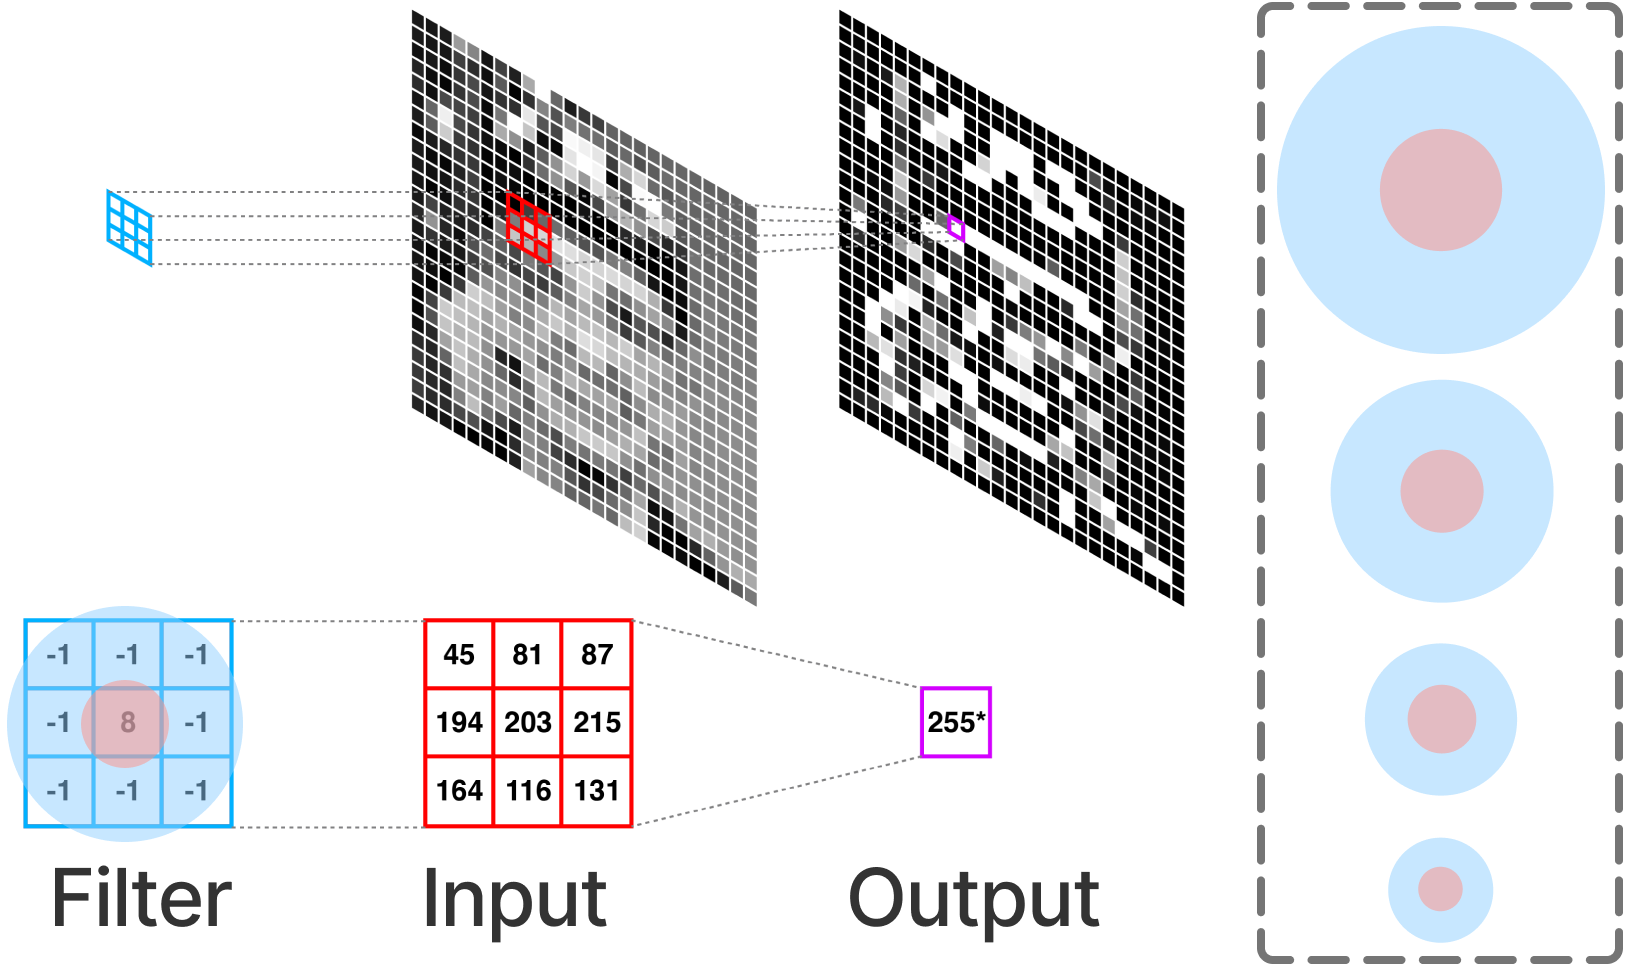
\includegraphics[width=0.7\linewidth]{media/convolution.png}
    \begin{minipage}{0.8\textwidth}
    \caption{
    Applying a convolution on an image is a common approach to model center surround
    fields. 
    % The convolution works by sliding a filter over an image and computing
    % the sum of element-wise multiplications to generate the output pixel. 
    Every pixel of the input image is multiplied with the center value of the filter (8)
    and then summed up with every surround pixel multiplied with the corresponding value
    in the filter (-1). The resulting sum is the new pixel value for the output image at
    the position of the original pixel. the left Figure is inspired by Gundersen
    \parencite*{Gundersen2017}. The right side shows a filterbank, existing of multiple
    filters in different sizes.}
    \label{fig:figure5}
    \end{minipage}
\end{figure}

To address the benefits of different sized center surround fields of the retina, it is
sufficient to create multiple filters of varying sizes. On the right in Figure
\ref{fig:figure5} a so called filterbank is shown. Each of the different sized filters
will be applied on the input image and generate its own output, similar to the sensory
channels of the visual system. Larger filters will compare more pixels and will respond
stronger to low spatial frequencies. Smaller filters will respond to high spatial
frequencies. The outputs from all the filters of a filterbank are representing the image
information decomposed by frequencies. In order to reconstruct the image, it is sufficient
to sum the filter outputs. The reconstructed image is identical to the original
image, since all information is kept during the process.

To replicate human perception the DOG (Difference Of Gaussian) model from Blakeslee and
McCourt does a reweighting of the filter outputs before reconstruction
\parencite{Blakeslee1997}. Inspired by the contrast sensitivity function of the human
visual system, it attenuates lower frequencies. As a consequence the output image is no
longer identical to the input image. In fact for the simultaneous contrast illusion the
left patch is brighter and the right patch is darker, aligning with the human perception
of the illusion.

\newpage

\begin{figure}[H]
    \centering
    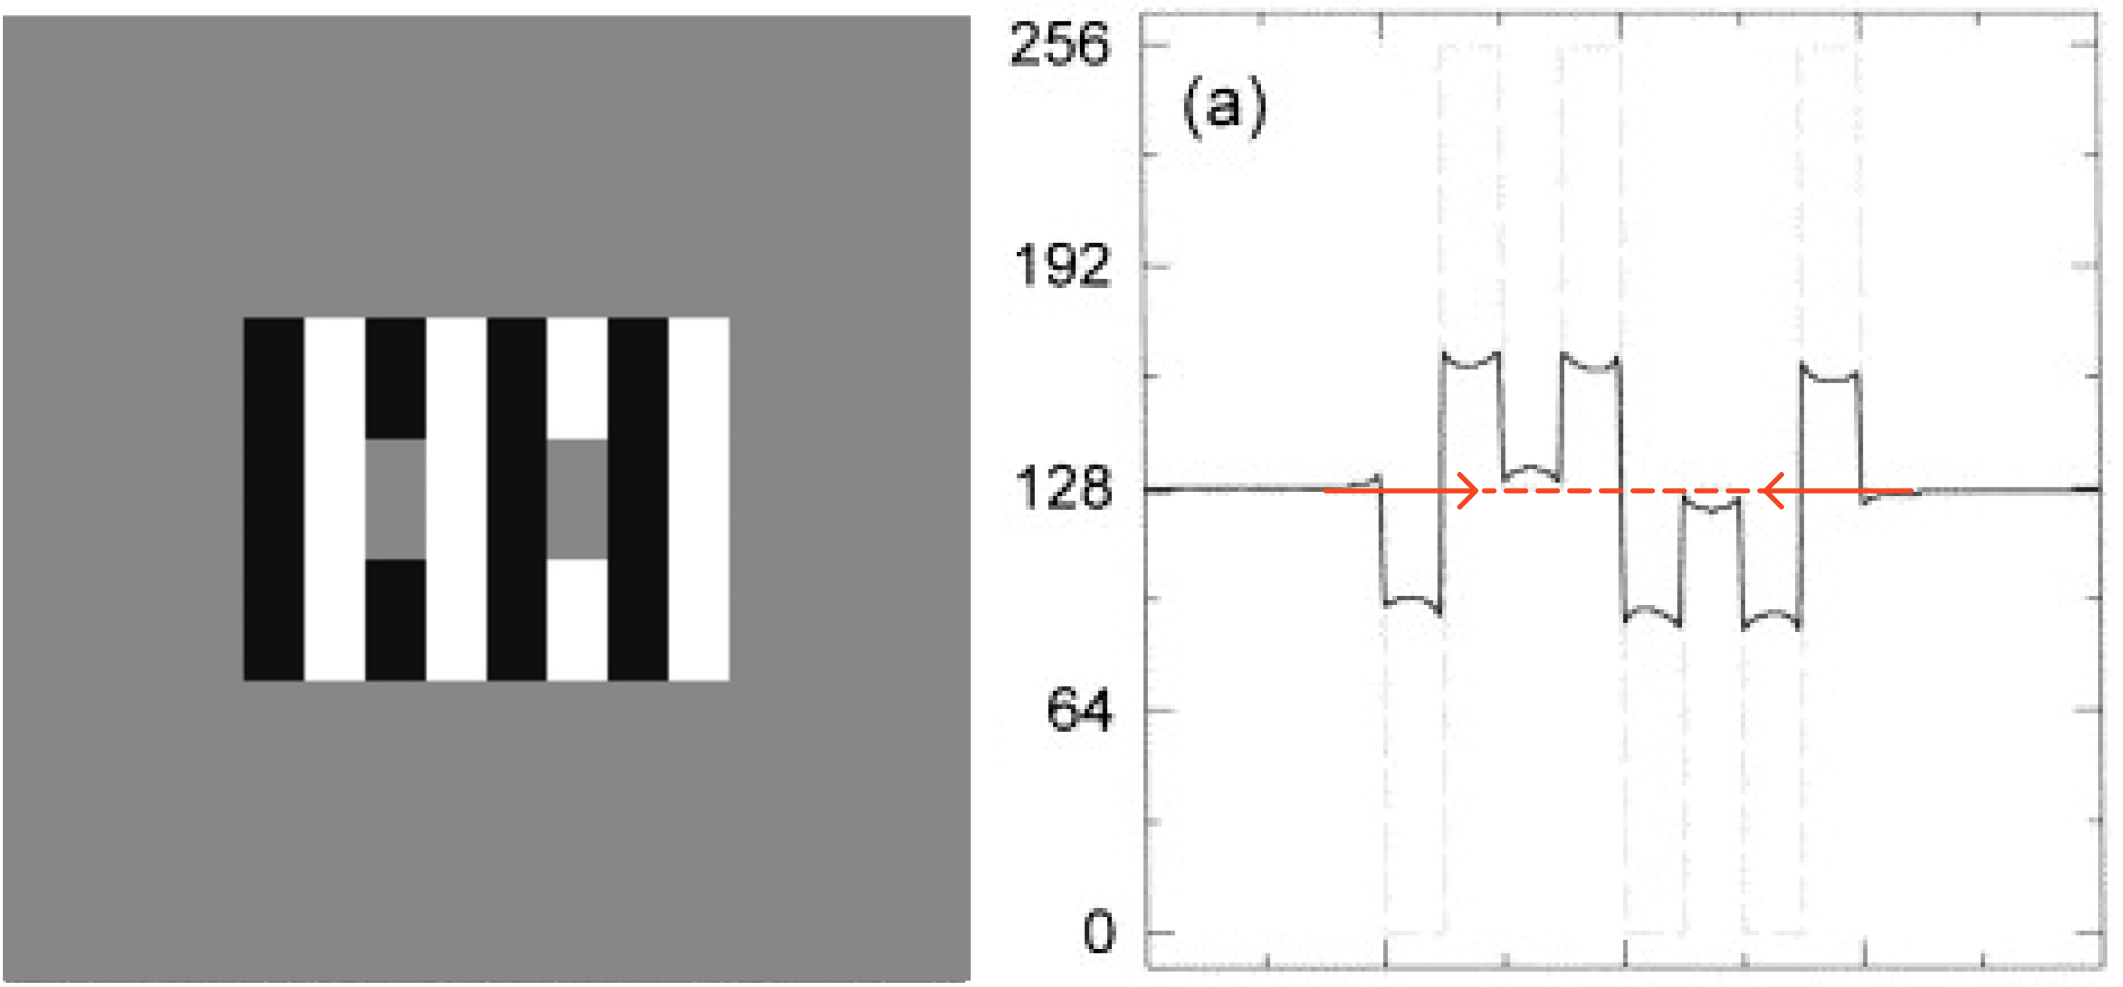
\includegraphics[width=0.7\linewidth]{media/whites_effect_model.png}
    \begin{minipage}{0.8\textwidth}
    \caption{In White's Effect (left) the shift in perceived brightness is in the opposite
    direction compared to brightness contrast. Both patches are identical, but the left
    patch on the black bar appears to be brighter than the patch on the white bar, even if
    it shares most of its edges with white surfaces \parencite{Whit1979}. The diagram on
    the right shows the processed White's Effect illusion by the ODOG model. The dashed
    line refers to the luminance profile across the horizontal center of the illusion. The
    solid line represents the models output along the same line. The red markers indicate
    that the models output is in accord with the human perception
    \parencite{Blakeslee1999}.}
    \label{fig:figure6}
    \end{minipage}
\end{figure}

The reweighting between decomposition and reconstruction appears to be a key mechanism of
the DOG model making it capable of replicating human perception of the simultaneous
contrast illusion. However, the DOG model cannot account for all brightness phenomena. For
instance, the White's effect, illustrated on the left side of Figure \ref{fig:figure6},
cannot be explained by Blakeslee and McCourt's initial model. One year later, in 1999,
they developed an extended version of the model, called ODOG (Oriented Difference Of
Gaussian), which can account for White's effect shown on the right side of Figure
\ref{fig:figure6} \parencite{Blakeslee1999}. Two changes are responsible for its new
capabilities. They extended the filterbank by six different orientations for each filter,
therefore they also changed the isotropic filters of the DOG model to anisotropic filters
in order to be able to rotate them. The second change is a normalization step before
reconstruction. The ODOG model will be discussed in more detail at a later point in the
thesis. \\
The ODOG model became very famous and inspired a whole family of so-called spatial
filtering models. Among them is a model with a different approach, the BIWaM (Brightness
Induction Wavelet Model) model from Otazu. It doesn't use a filterbank to decompose the
image, but rather convolves its filters within a wavelet transformation
\parencite{Otazu2008}.


\subsection{ODOG and BIWaM}

ODOG and BIWaM are oriented spatial-filtering models, highlighting the importance of
low-level vision. Both models process an input image using filters, which are inspired by
the center surround fields. As shown in Figure \ref{fig:figure7}, their processing begins
with the decomposition of the input image (Step 1), using spatially scaled and oriented
filters. Each filter results in an channel that captures different orientations and
spatial frequencies of the image. The channels are then processed (Step 2) by reweighting
and normalization, each model has it own strategy. In the final step (Step 3) all outputs
are merged to reconstruct the output image.

\begin{figure}[H]
    \centering
    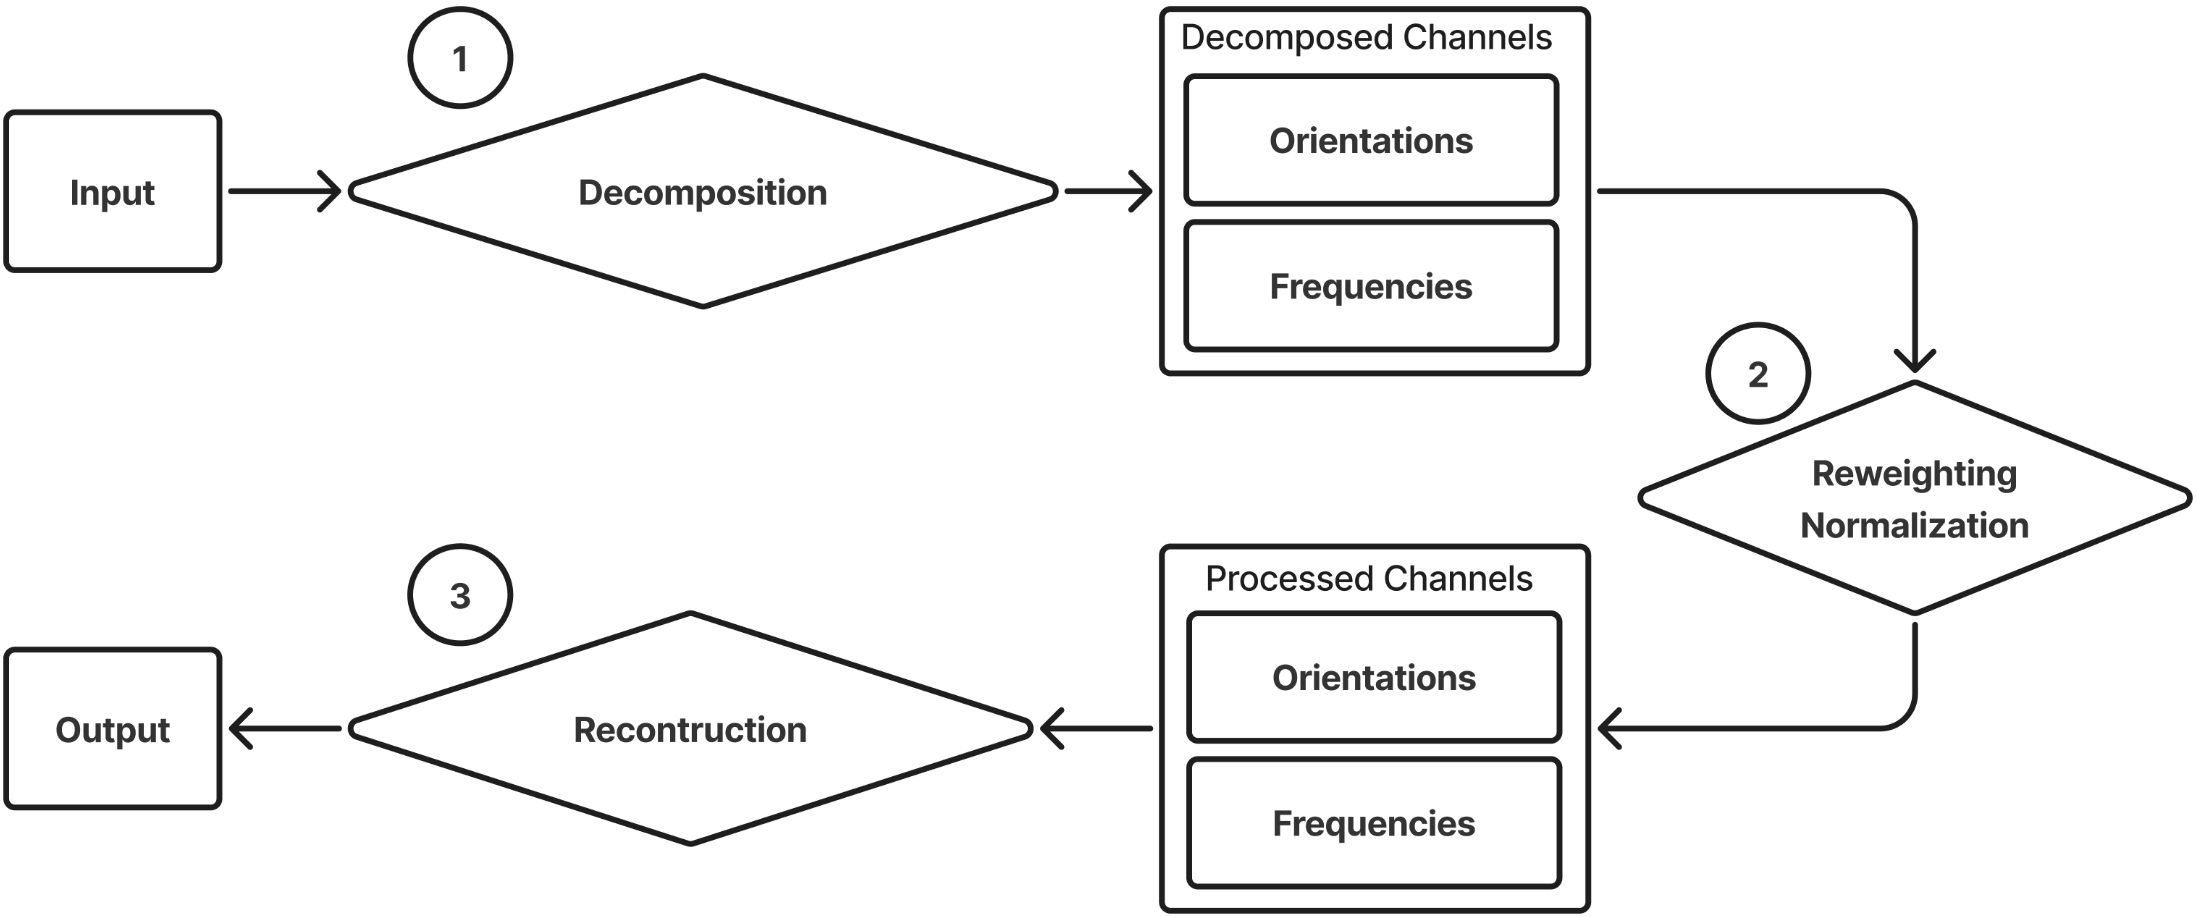
\includegraphics[width=\linewidth]{media/model_structure.png}
    \begin{minipage}{0.8\textwidth}
    \caption{Structural overview of ODOG and BIWaM models, three steps to analyze}
    \label{fig:figure7}
    \end{minipage}
\end{figure}

The ODOG model uses a filterbank consisting of 42 filters in seven different scales and
six different orientations. These filters are applied on the input image by a convolution
for every filter, to create the frequency specific and oriented channels. The outputs of
the filters within the same orientation are summed, with weights that are determined by
the spatial frequency. Lower frequencies receive smaller weights than higher frequencies,
similar to the contrast sensitivity of the visual system. These responses are normalized
by their root-mean-square energy, which is computed across all pixels and summed to
yield the model output. As a consequence of the response normalization, orientations with
little energy in the input image will have a proportionally larger influence on the model
output \parencite{Betz2015}.

For the decomposition in the BIWaM model, a wavelet transformation is used instead of a
filterbank. This wavelet transformation also performs convolutions with different filters.
Only three orientations are used, but a wider range of scales from 1 cpd (cycles per
degree) to the Nyquist frequency. It iterates through the decomposition recursively,
downsampling the image at each iteration but using the same filter. Therefore, it
generates channels for different filter-to-image scales in each iteration, similar to the
ODOG model. After decomposition, all channels are reweighted by a function that is also
inspired by the contrast sensitivity function of the visual system. For normalization,
they use factors generated for specific areas of the image, resulting in a local
normalization. This could be a main difference between the models \parencite{Betz2015}. In
the final step, the BIWaM model merges the filter outputs to generate the output image.


ODOG and BIWAM may seem different at first glance, because of their distinct processing
techniques. But some processes are similar to those in the other model. What exactly is
making a difference? Is the decomposition and reconstruction interchangeably in both
models, does the processing on the channels make the difference? These questions arise
when dealing with both models and are the focus of this thesis.  The aim is to explore
whether they process identical information as a subset of the other, or if they address
distinct concepts.

\newpage


\section{Research}

A review of the publications revealed differences between the models, as listed in the
table in Figure \ref{fig:figure8}. To understand their impact, the plans in the next
subsection are being developed.

\subsection{Methods}

For each step shown in Figure \ref{fig:figure7}, the focus will be on the structural
differences between the models. Adjusting the ODOG model to align it more closely with the
BIWaM model, will reveal their importance step by step, shown in the diagram of Figure
\ref{fig:figure8}. The plan is to modify the source code for each part listed in the table
of Figure \ref*{fig:figure8} and to conclude every change by running the models with the
modification on a set of illusions and comparing the outputs quantitatively.

\begin{figure}[H]
    \centering
    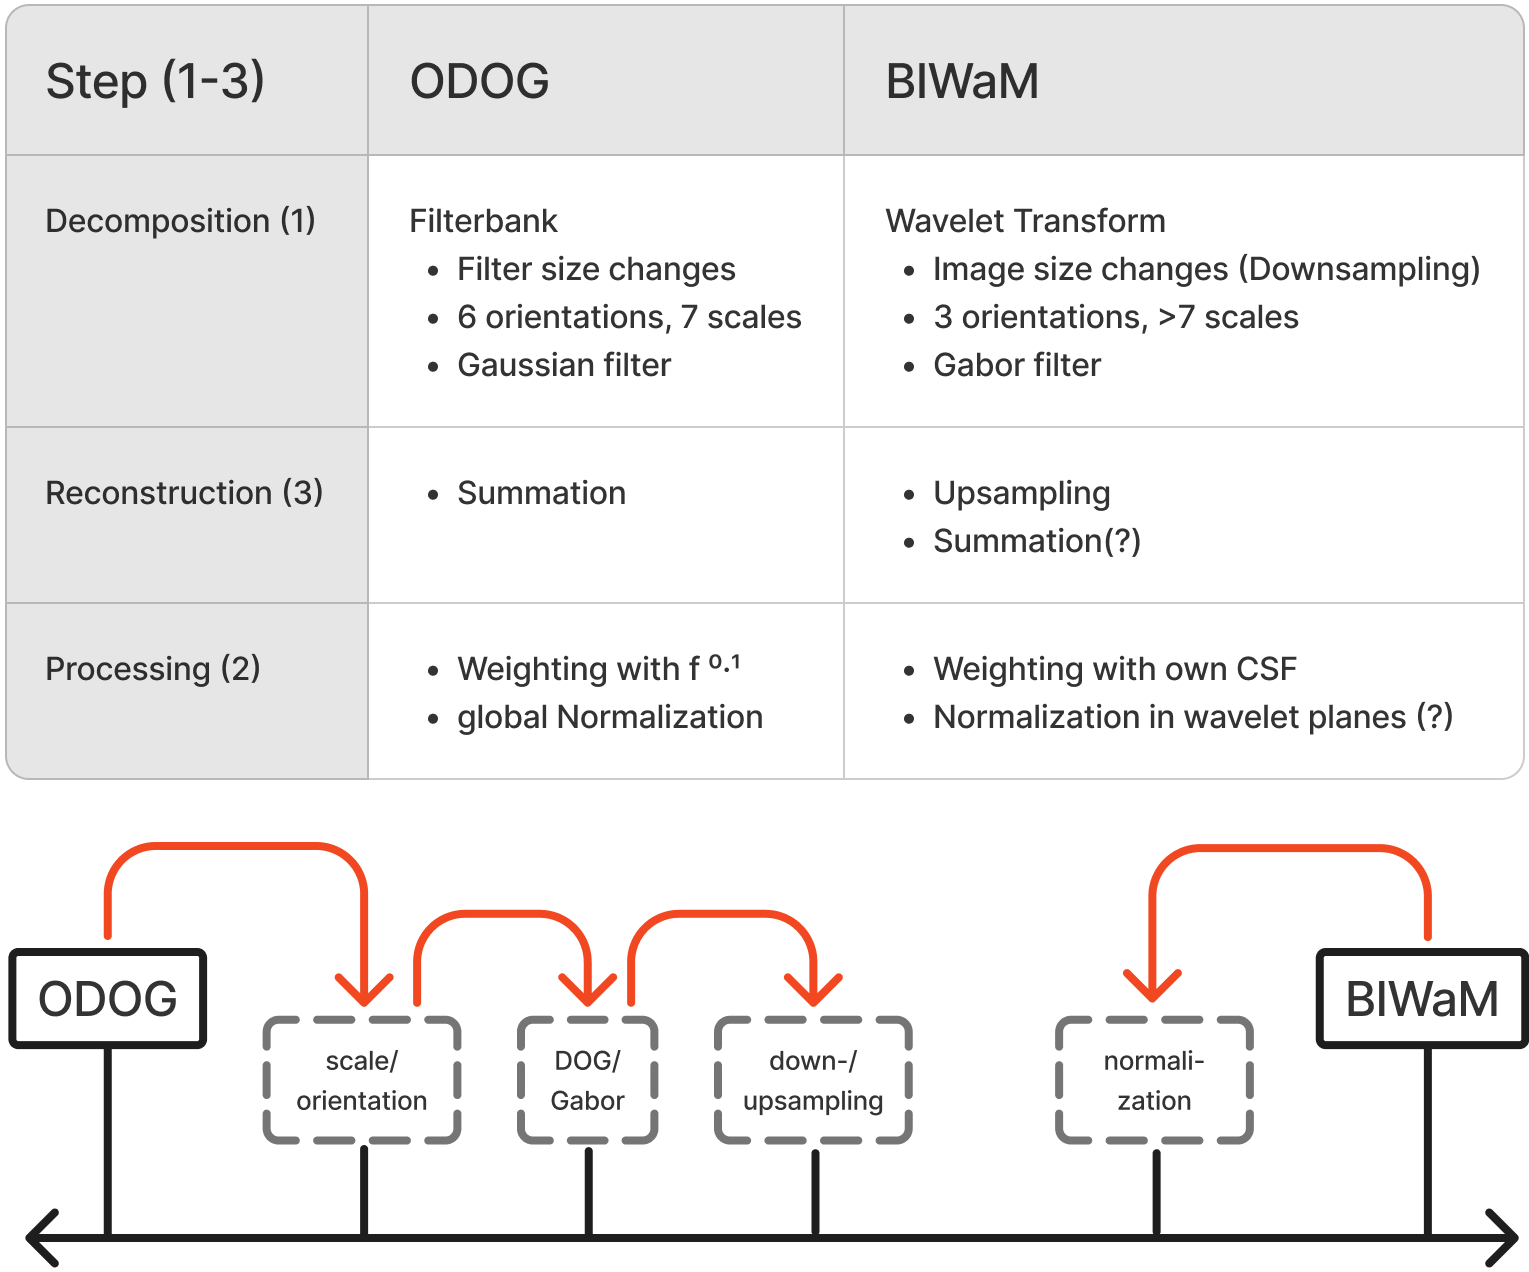
\includegraphics[width=\linewidth]{media/table_differences.png}
    \begin{minipage}{0.8\textwidth}
    \caption{The table shows the already known differences between the models for each of
    the steps (1-3). The diagram below shows how i plan to narrow down the search for
    differences. By adjusting the models for each of the steps shown and concluding the
    impact by comparing the output, I wat to isolate the differences with the most
    impact.}
    \label{fig:figure8}
    \end{minipage}
\end{figure}

\newpage

\subsection*{Decomposition and Reconstruction}
\begin{enumerate}
    % \item For decomposition we plan to change the ODOG model stepwise. For example
    % changing the filterbank size, to match the orientations and scales of the BIWaM. Also
    % do this adjustment for the type of filter used in the convolutions and try to copy the
    % downsampling instead of the different filter sizes.
    \item A wavelet transformation results in a function that is localized in both space
    and frequency. In the ODOG model the results of the filterbank will hold every spatial
    data for any frequency, in other words the responses of different frequencies will be
    a two-dimensional image itself, where the value at each pixel correlates to the
    presence of this frequency at this location. Can we find any details about wavelet
    transformation being the superior?
    \item Looking at the functions used for convolution (Gabor and Difference of Gaussian)
    and change them in the source code could be informative.
    \item The levels of decomposition in the wavelet transformation can be compared to
    the filterbank size. Adjusting them will show the influence in decomposition and the
    difference between the models.
    \item The BIWaM uses a reverse wavelet transformation to reconstruct the output image,
    while the ODOG is summing up the channels it created during decomposition and
    processing stage. Where is the difference and could changing the source code show
    the differences to the processes?
\end{enumerate}


\subsection*{Processing}
\begin{enumerate}
    \item To analyze the processing step for both models, it will be necessary to look at
    processing inside the wavelet planes versus processing in the filterbank output.
    Separatly to the processing itself, does it make a difference to compute the
    decomposed image inside a wavelet plane versus inside the filterbank channels?
    \item The processing itself is different independent from where it is happening. Does
    the weighting in BIWaM really make a difference to the one the ODOG is using? To
    investigate this, a modification of the source code is necessary, e.g. changing the
    implementation of BIWaM and use a $f^{0.1}$ function to attenuate low frequencies,
    like in the ODOG model.
    \item According to Otazu et al., \emph{"this modified CSF takes into account the
    (spatial) surround information, so that the value of the contrast sensitivity
    increases when surround contrast decreases and vice versa."}, \parencite{Otazu2008}.
    But aren't low frequencies filters applying the same logic? Kingdom mentioned:
    \emph{"In multiscale spatial-filtering models remote context makes its impact via the
    coarse-scale (low-spatial-frequency) filters"}
    \parencite{Kingdom2014}
\end{enumerate}


\newpage

\section{Structure of the thesis}


\begin{enumerate} 
    \item Introduction
    \begin{enumerate}
        \item Light an the Visual System
        \item Low-Level Vision
        \item Modelling Human Vision
        \item ODOG and BIWaM
    \end{enumerate}
    
\end{enumerate}


\newpage

\section{Methods}  %\newline \textit{One of the following will be in focus} 
    \begin{enumerate}
        \item \textbf{Recreation of published predictions for BIWaM}
        \begin{itemize}
            \item Understanding the algorithm and parameter exploration.
            \item Python reimplementation, to compare with ODOGs python implementation.
            \item Recreate input stimuli from the paper using the Stimupy library.
            \item Evaluate robustness of the BIWaM model to input variations.
            \item Illusions tested: Two versions of SBC, two versions of White’s effect, and the Todorovic illusion.
        \end{itemize}
    
        \item \textbf{Modification of parameters} \newline BIWaM:
        \begin{itemize} 
            \item CSF parameters
            \item Decomposition levels, window size, peak s.f.
            \item A big window size does effectively end up in global normalization (?)
            \item Wavelet filter functions (?)
        \end{itemize}
        ODOG:
        \begin{itemize} 
            \item Number of scales and orientations 
            \item Filter functions
            \item Down- and upsampling (?)
        \end{itemize}
    
        \item \textbf{Comparative testing}:
        \begin{itemize}
            \item Applied both models to recreated stimuli and analyze outputs.
            \item Adjusted parameters to align both models for direct comparison.
        \end{itemize}
    \end{enumerate}

\newpage

\section{Results} 
\begin{enumerate}
    
    \item \textbf{Recreation of published predictions for BIWaM}:
    \begin{itemize}
        \item Avilable Matlab implementation is another version (CIWaM).
        \item Bad reproducibility led to extensive research and parameter exploration.
        \item DWT function is highly optimized and undocumented -> took a lot of time to understand.
        \item Python reimplementation behaves same as Matlab version (CIWaM).
        \item Using CIWaM\_per\_channel function from CIWaM code as BIWaM representative.
        \item \textbf{Predictions}
            \begin{itemize} 
                \item Available BIWaM predicts brightness illusions qualitatively, but not quantitatively.
                \item Model outputs diverged from published results despite wide parameter adjustments.
                \item This led to the question of whether the available model is different, or whether the parameters are different, or whether the re-created stimuli (as input) are different.
                \item Tests indicated high robustness of BIWaM to input variations, suggesting that output differences are coming from differences in implementation rather than the re-created stimuli.
            \end{itemize}
    \end{itemize}
    
    \item \textbf{Findings on parameter effects}:
    \begin{itemize}
        \item Adjusting wavelet levels influenced decomposition depth but did not resolve discrepancies.
        \item Modifying filters results in ...
        \item Modifying window size results in ...
        \item Modifying peak s.f. results in ...
    \end{itemize}

    \item \textbf{Findings on comparative testing}:
    \begin{itemize}
        \item On the exact same stimuli the original models ....
        \item With aligned parameters both models behave ...
    \end{itemize}

    \item \textbf{Potential differences between models}:
    \begin{itemize}
        \item Studying the models showed that the following features of the models are causing differences
    \end{itemize}

\end{enumerate}

\newpage

\section{Discussion} 
\begin{enumerate}
    \item \textbf{Linking differences in structure with results in behavior}
    \item \textbf{Insights into decomposition}:
    \begin{itemize}
        \item Information loss through downsampling does not appear to cause output differences.
    \end{itemize}
\end{enumerate}



\newpage
\nocite{Adelson1996}
\nocite{Brainard2003-BRACCD-2}
\nocite{Hanson1978}
\nocite{Murray2021}
\nocite{Kingdom2014}
\nocite{Robinson2007}
\vspace*{1cm}
%Literatur
\begin{minipage}{1\textwidth}
\printbibliography
\end{minipage}


\end{document}
